\section{Modelo cliente-servidor/sistema web}

Em um modelo cliente-servidor, os dados de um sistema são armazenados em poderosos computadores chamados servidores. Os usuário utilizam máquinas mais simples, chamadas de clientes. As máquinas cliente e servidor são conectadas entre si por uma rede, conforme ilustrado pela Fig. \ref{cliente_servidor}.

\begin{figure}[H]
\centering
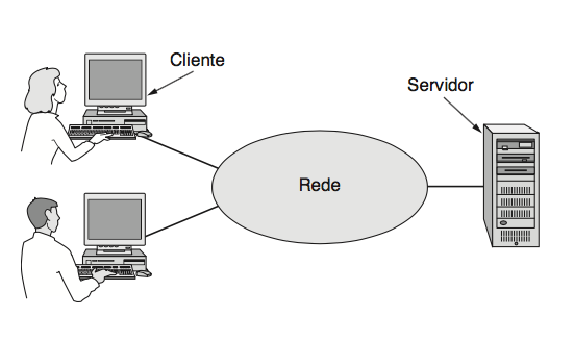
\includegraphics[width=8cm]{figuras/cliente_servidor.eps}
\caption{Modelo cliente-servidor.}\label{cliente_servidor}
\end{figure}

Em uma aplicação web, o servidor fornece páginas Web com base em seu banco de dados em resposta a solicitação do cliente. Sob a maioria das condições, um único servidor pode lidar com um grande número (centenas ou milhares) de clientes simultaneamente.

Examinando o modelo cliente-servidor em detalhes, é possível perceber que existem dois processos em execução, um na máquina cliente e outro na máquina servidor. A comunicação toma a forma do processo cliente enviando uma mensagem pela rede ao processo servidor. Então, o processo cliente espera por uma mensagem de resposta. Quando processo servidor recebe a solicitação, ele executa o trabalho solicitado ou procura pelos dados solicitados e envia uma resposta de volta (Fig. ) (TENENBAUM, 2011).

\begin{figure}[H]
\centering
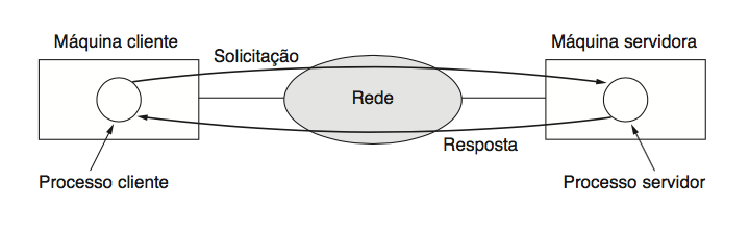
\includegraphics[width=10cm]{figuras/cliente_servidor_mensagens.eps}
\caption{Mensagens trocadas entre um processo cliente e um processo servidor}
\end{figure}

\section{Framework Django}

Django é um framework gratuito e de código aberto para a criação de aplicações web, escrito em Python, uma linguagem de programação multiparadigma. É um framework web, ou seja, é um conjunto de componentes que ajuda a desenvolver sites de forma mais rápida e mais fácil.

Quando se está construindo um site, o desenvolvedor sempre precisa de um conjunto similar de componentes: uma maneira de lidar com a autenticação do usuário (inscrever-se, realizar login, realizar logout), painel de gerenciamento para o seu site, formulários, upload de arquivos, etc. Há muito tempo, outras pessoas notaram várias semelhanças nos problemas enfrentados pelos desenvolvedores web quando estão criando um novo site, então eles uniram-se e criaram os frameworks (Django é um deles) que lhe dão componentes prontos, que você pode usar. O framework Django utiliza o padrão MTV (model-template-view), onde as views funcionam como controllers e templates funcionam como views. 

\section{Sistema interno}

Sistema responsável por se comunicar com o aparato eletrônico, recebendo dados e interpretá-los. Para isso, será utilizado a linguagem de programação C++. C++ é uma linguagem de programação de alto nível com facilidades para o uso em baixo nível. Foi desenvolvida por Bjarne Stroustrup (foto) como uma melhoria da linguagem C, e desde os anos 1990 é uma das linguagens mais populares do mundo.

Alguns profissionais afirmam que C++ é a linguagem mais poderosa que existe, veja algumas características dela:

\begin{itemize}
\item É um superconjunto da linguagem C, e contém vários melhoramentos;
\item É a porta para a programação orientada a objetos;
\item C++ pode virtualmente ser efetivamente aplicado a qualquer tarefa de programação;
\item Há vários compiladores para diversas plataformas tornando a linguagem uma opção para programas multiplataforma.
\end{itemize}

